\textit{Clusterapp} es la herramienta desarrollada para cumplir los objetivos de este trabajo.
Fue programada empleando el lenguaje de programación \textit{Python}\footnote{https://python.org/} en su versión 3.5;
la decisión se motivó en la flexibilidad del lenguaje y la existencia en este de librerías científicas de reconocido prestigio, adecuadas para su aplicación en este trabajo.

Como se mencionó inicialmente en este capítulo, se tuvo en cuenta al implementar la herramienta que no todos sus usuarios dispondrían de iguales conocimientos computacionales.
Es por ello que se desarrollaron tres variantes para la interacción de los usuarios con la aplicación, cada una adaptada a un perfil de usuario específico.

\subsection{Interfaz web}\label{subsec:interfazWeb}

La interfaz web provee a los usuarios más generales de una variante visual para interactuar con la herramienta.
Los resultados que produce se muestran a través de gráficos y tablas directamente en pantalla, lo que simplifica su análisis.

Para la implementación de esta interfaz se utilizó el framework \textit{Flask}\footnote{http://flask.pocoo.org/}, por su simpleza, velocidad y versatilidad.

En este modo se ofrecen dos vistas diferentes:

\begin{itemize}
    \item \textbf{Análisis de datos}: Vista enfocada al análisis de los patrones existentes en el conjunto de datos y los resultados producidos por diferentes algoritmos de clustering al aplicarse con determinadas configuraciones y características de audio. Puede observarse un ejemplo de esta vista en la figura~\ref{img:dataset-analysis}
    \item \textbf{Selección de las mejores características}: Esta vista permite determinar el conjunto de características de audio para el que se produce el resultado de mejor evaluación para determinado algoritmo de clustering. Un ejemplo de esta vista aparece en la figura~\ref{img:best-features}.
\end{itemize}

\begin{figure}[!h]
    \centering
    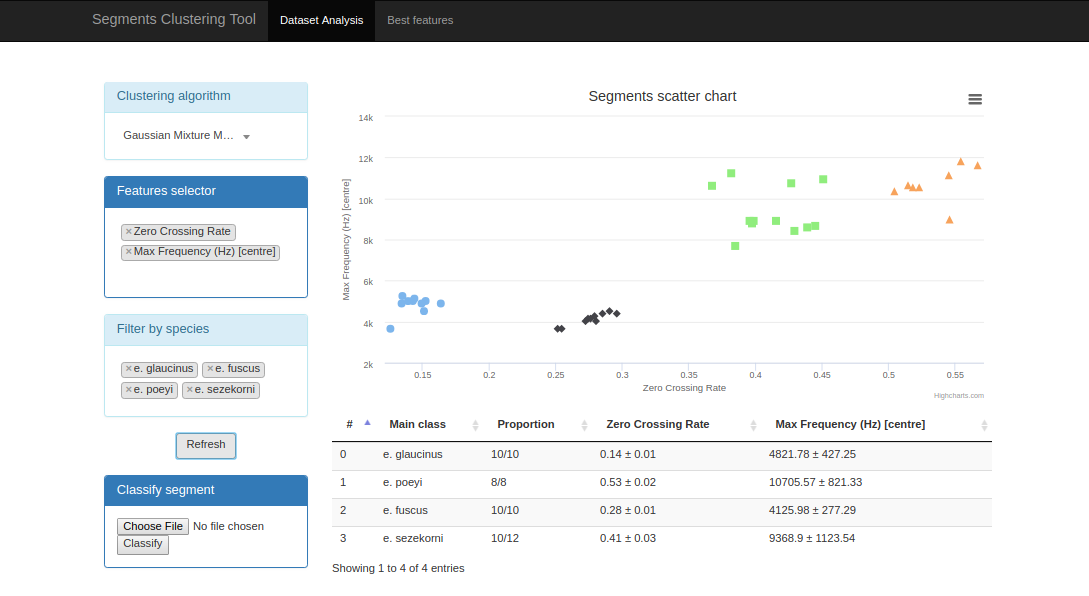
\includegraphics[width=\textwidth]{dataset-analysis.png}
    \caption{Vista de análisis de datos de la interfaz web de la herramienta \textit{Clusterapp}.}
    \label{img:dataset-analysis}
\end{figure}

\begin{figure}[!h]
    \centering
    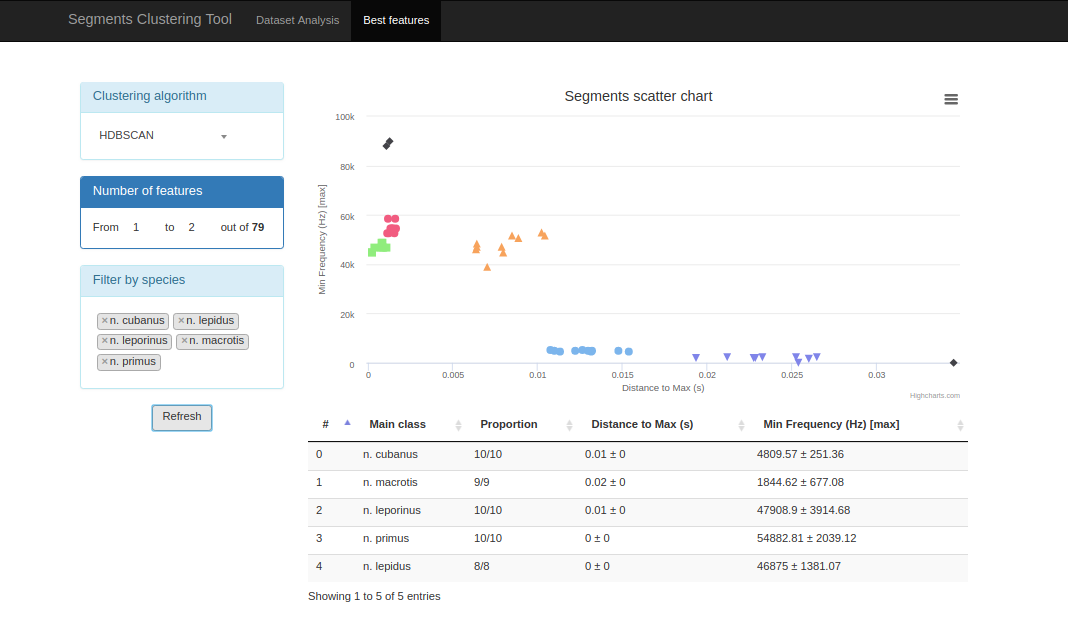
\includegraphics[width=\textwidth]{best-features.png}
    \caption{Vista de selección de las mejores características, de la interfaz web de la herramienta \textit{Clusterapp}.}
    \label{img:best-features}
\end{figure}

Las opciones de configuración en la interfaz web, así como la presentación de los resultados, varían en dependencia de si se dispone o no de información sobre la clasificación real de los segmentos de audio del conjunto de datos sobre el que se realiza el análisis.
Asimismo, en concordancia con dicha información se elige si será supervisado o no, el método para evaluar la calidad de los resultados de los algoritmos;
que es usado en la selección de las características que mejor diferencian los distintos tipos de vocalizaciones presentes en el conjunto de datos.

\subsection{Interfaz de línea de comandos}\label{subsec:CLI}

\subsection{Librería de Python}\label{subsec:libreríaDePython}
